\subsection*{Single Shot MultiBox Detector}

Zwar liefern die oben genannten Objektdetektoren akkurate Ergebnisse, allerdings sind sie als zu rechenintensiv und langsam einzuordnen, als dass sie für Echtzeit Applikationen eingesetzt werden könnten. Der \textit{Single Shot MultiBox Detector} (SSD) unterscheidet sich von vorhergehenden Modellen, wie beispielsweise den R-CNN Detektoren, dahingehend, dass er bewusst auf den Schritt der Generierung von Bounding Box Vorschlägen und des \textit{Poolings} verzichtet, um wesentlich schneller ablaufen zu können als andere Objektdetektoren. Die Präzision der Klassifikationen bleibt hierbei erhalten, selbst Bilder niedriger Auflösung können weiterhin verarbeitet werden. Dem \textit{SSD} genügt also ein einziges tiefes neuronales Netz zum Lokalisieren und Klassifizieren von Objekten. Wie der \textit{SSD} aufgebaut ist und welche Ansätze er verfolgt, soll in diesem Unterkapitel erläutert werden \cite{ssd.20161229}. 

\begin{figure}[ht]
	\begin{center}
		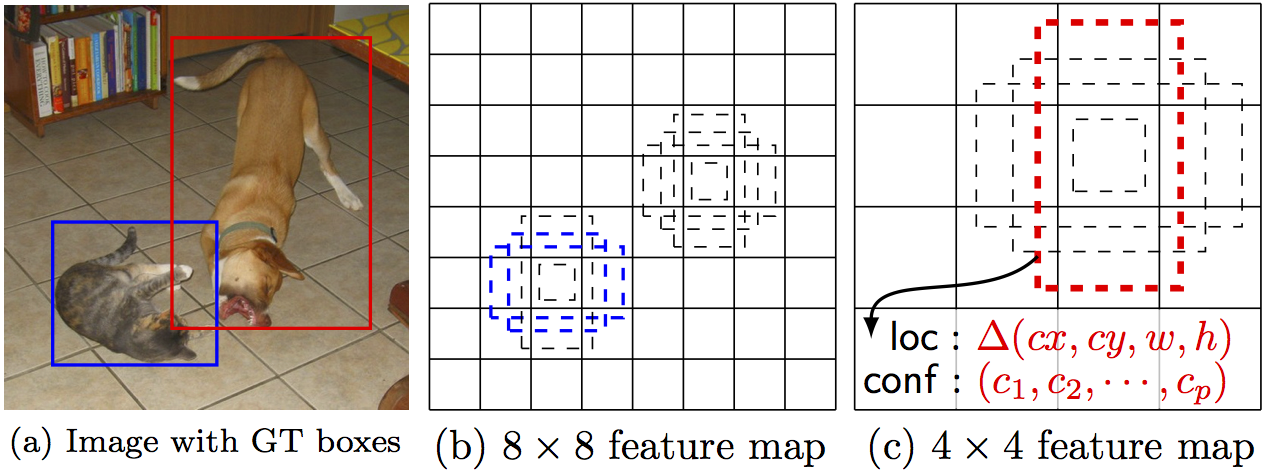
\includegraphics[width=15cm]{Bilder/ssd_framework.png} 
		\caption[SSD Bounding Box Proposals]{SSD Bounding Box Proposals \cite{ssd.20161229}}
		\label{framework}
	\end{center}
\end{figure}

Die Architektur des \textit{SSD} zielt darauf ab, durch unterschiedlich große \textit{Convolutional Layer} \textit{Feature Maps} unterschiedlicher Skalierung in die Klassifikation mit einfließen zu lassen. Anschaulich kann es sich vorgestellt werden, als werde das Bild in mehrere unterschiedlich große Gitterstrukturen unterteilt und die resultierenden Zellen jeweils einzeln klassifiziert. Dadurch ist es möglich, Objekte unterschiedlicher Größe zu erkennen. Für jede Zelle im Gitter wird eine gleiche Anzahl vordefinierter Bounding Boxen, die unterschiedliche Seitenverhältnisse aufweisen, definiert. Daher entstammt der Name \glqq MultiBox\grqq{}. Abbildung \ref{framework} zeigt beispielsweise, wie eine Katze (in blau) und ein im Vergleich zur Katze größerer Hund (in rot) durch unterschiedlich große Gittereinteilungen und Bounding Box Seitenverhältnisse detektiert werden. Durch die \textit{MultiBox} Eigenschaft wird ebenso sichergestellt, dass sowohl horizontal als auch vertikal ausgeprägte Objekte in der selben Zelle gleichzeitig erkannt werden können (siehe Abbildung \ref{boundingboxes}) \cite{ssd.20161229}.

\begin{figure}[ht]
	\begin{center}
		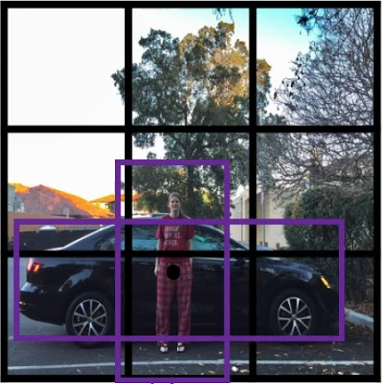
\includegraphics[width=7cm]{Bilder/bounding_boxes.png} 
		\caption[Bounding Boxes]{Bounding Boxes \cite{AndrewNg.2019}}
		\label{boundingboxes}
	\end{center}
\end{figure}

Für jede dieser Bounding Boxen bestimmt der \textit{SSD} Wahrscheinlichkeiten für Klassenzugehörigkeiten als auch Verschiebungen der vordefinierten Bounding Box zur wahren Bounding Box des Objekts für jede Klasse. Die Kostenfunktion ist durch die gewichtete Summe des Lokalisationsverlustes und des Klassifikationsverlustes bestimmt. Während der Klassifikationverlust durch eine Softmax-Funktion bestimmt werden kann, wird der Lokalisationsverlust über die \textit{Smooth L1} Funktion (\ref{smooth}) bestimmt. Der Parameter $l$ beschreibt die vorhergesagte Bounding Box, der Parameter $g$ die originale Bounding Box nach den Trainingsdaten \cite{ssd.20161229}.

\begin{equation}\label{smooth}
\begin{split}
L_{loc}(l^j,g) = \sum\limits_{j \in Pos}^{n} \sum\limits_{i \in (x,y,w,h)}^{m} SM_{L1}(l^j_i - g_i) \\
SM_{L1}(l^j_i - g_i) = \begin{cases}
							0.5x^2      & \text{wenn } |x| < 1\\
							|x| - 0.5   & \text{sonst}
						   \end{cases}
\end{split}
\end{equation}
\equations{Die Smooth L1 Funktion}

\begin{figure}[ht]
	\begin{center}
		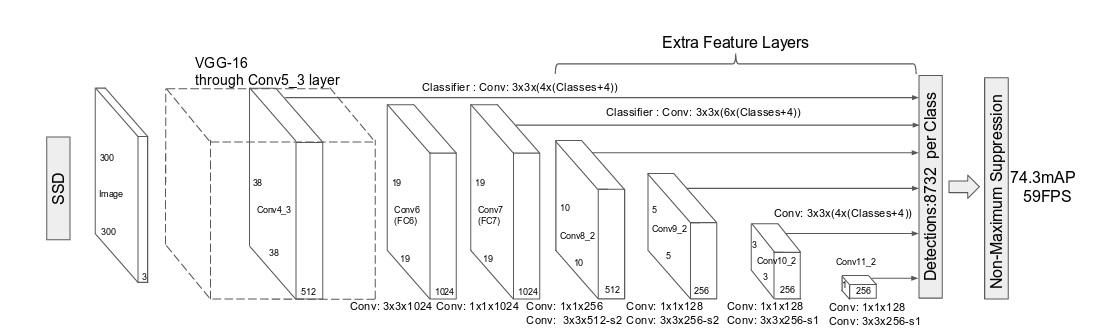
\includegraphics[width=15cm]{Bilder/ssd_architecture.png} 
		\caption[SSD Architektur]{SSD Architektur \cite{ssd.20161229}}
		\label{architecture}
	\end{center}
\end{figure}

Technisch basiert der \textit{SSD} auf der Idee eines \textit{Feed-Forward Convolutional Networks} (siehe Abbildung \ref{architecture}). Er benutzt ein \textit{VGG-16} Basis Netzwerk\footnote{\textit{VGG-16} ist ein auf dem Datensatz von \textit{ImageNet} basierendes neuronales Netz, das bis zu 1000 unterschiedliche Kategorien klassifizieren kann \cite{MathWorks.2019b}.}, dessen \textit{Fully-Connected Layer} am Ende entfernt wurden. Die resultierende \textit{Feature Map} wird nun einer Reihe von ständig kleiner werdenden \textit{Convolutional Layern} unterzogen. Jedes \textit{Convolutional Layer} kann eine feste Anzahl an Detektionen bestimmen. Eine Detektion wird durch eine Klassenangabe und die Lage einer vorhergesagten Bounding Box bestimmt. Eine Bounding Box wird wie bereits erläutert durch den linken oberen Eckpunkt $P(x,y)$ und eine Höhe und Breite bestimmt. Bei $c$ Klassen hat der \textit{Feature Vektor} einer Detektion demnach die Größe $c+4$. Bei einer \textit{Feature Map} Größe von $m x n$ und $k$ verschiedenen vordefinierten Bounding Boxen ergeben sich also $m \cdot n \cdot k \cdot (c+4)$ verschiedene \textit{Feature Vektoren} für eine Feature Map \cite{ssd.20161229}. Diese \textit{Feature Vektoren} werden nun an das Ende des Netzes zur Klassifikation weitergeleitet.

Dieser Vorgang wird für alle \textit{Feature Maps} für alle \textit{Convolutional Layer} durchgeführt. Die daraus folgende Menge an Detektionen wird durch ein \textit{Non Maximum Suppression Layer} in ihrer Größe reduziert. Als Maß zur Filterung wird die \textit{IoU} der detektierten Bounding Box zur wahren Bounding Box verwendet. Überschreitet diese einen Wert von 0.5, so ist diese der originalen Bounding Box zugeordnet. Demnach ist es auch möglich, dass eine originale Bounding Box mehreren vordefinierten Bounding Boxen zugeordnet werden kann \cite{ssd.20161229}.

Während des Trainingsprozesses des \textit{SSD300}\footnote{SSD300 verwendet Bilder der Auflösung 300x300 Pixel. Alternativ existiert ebenso SSD512 für Bilder der Auflösung 512x512 Pixel. Die Bilder können jedoch auch kleiner als die vorgegebene Auflösung gewählt werden.} wurde eine Lernrate von $\eta = 10^{-3}$ für das Mini-Batch Verfahren mit Batchgröße 32 und Moment $\beta = 0.9$ verwendet. Die Gewichtungen wurden \textit{Xavier} initialisiert. Nach 40.000 Iterationen wurde die Lernrate für 10.000 Iterationen auf $\eta = 10^{-4}$ reduziert und schließlich auf $\eta = 10^{-5}$ \cite{ssd.20161229}. Auf Basis der PASCAL VOC Datensätze aus 2007 und 2012 wurde mit dieser Konfiguration eine \textit{mAP} von 74.3\% für SSD300 respektive 76.8\% für SSD512 erreicht.
